% ANUfinalexam.tex (Version 2.0)
% ===============================================================================
% Australian National University Final Exam LaTeX template.
% 2004; 2009, Timothy Kam, ANU School of Economics
% Licence type: Free as defined in the GNU General Public Licence: http://www.gnu.org/licenses/gpl.html

\documentclass[a4paper,10pt,leqno]{article}
\usepackage[fleqn]{mathtools}
\usepackage[labelformat=empty]{caption}
\usepackage{fancyhdr}
\usepackage{float}
\usepackage{tikz}
\usetikzlibrary{shapes}

% Insert your course information here %%%%%%%%%%%%%%%%%%%%%%%%%%%%%%%%%%

\newcommand{\institution}{UNIVERSITY OF THE PHILIPPINES DILIMAN}
\newcommand{\titlehd}{Database Systems}
\newcommand{\examtype}{Second Exam}
\newcommand{\examdate}{March 15, 2014}
\newcommand{\examcode}{CS165}
\newcommand{\writetime}{THREE Hours}
\newcommand{\lastwords}{End of Exam}

%%%%%%%%%%%%%%%%%%%%%%%%%%%%%%%%%%%%%%%%%%%%%%%%%%%%

% ANU Exams Office mandated margins and footer style
\setlength{\topmargin}{0cm}
\setlength{\textheight}{9.25in}
\setlength{\oddsidemargin}{0.0in}
\setlength{\evensidemargin}{0.0in}
\setlength{\textwidth}{16cm}
\pagestyle{fancy}
\lhead{} 
\chead{} 
\rhead{} 
\lfoot{} 
\cfoot{\footnotesize{Page \thepage \ of \pageref{finalpage} -- \titlehd \ (\examcode)}} 
\rfoot{} 

% DEPRECATED: ANU Exams Office mandated margins and footer style
%\setlength{\topmargin}{0cm}
%\setlength{\textheight}{9.25in}
%\setlength{\oddsidemargin}{0.0in}
%\setlength{\evensidemargin}{0.0in}
%\setlength{\textwidth}{16cm}
%\pagestyle{fancy}
%\lhead{} %left of the header
%\chead{} %center of the header
%\rhead{} %right of the header
%\lfoot{} %left of the footer
%\cfoot{} %center of the footer
%\rfoot{Page \ \thepage \ of \ \pageref{finalpage} \\
%       \texttt{\examcode}} %Print the page number in the right footer

\renewcommand{\headrulewidth}{0pt} %Do not print a rule below the header
\renewcommand{\footrulewidth}{0pt}

\begin{document}

% Title page

\begin{center}
%\vspace{5cm}
\large\textbf{\institution}
\end{center}
\vspace{1cm}

\begin{center}
\textit{ \examtype -- \examdate}
\end{center}
\vspace{1cm}

\begin{center}
\large\textbf{\titlehd}
\end{center}

\begin{center}
\large\textbf{\examcode}
\end{center}
\vspace{4cm}

\begin{center}
\textit{Writing Time:  \writetime}
\end{center}

% End title page

\newpage
\noindent{\textbf{Section 1: True or False [10 points]}\\\\}
\noindent Write {\textbf T} if the statement is true. If the statement is false, write {\textbf F}.

\noindent 1. Higher normal forms have more redundancy. \\
\noindent 2. In 3NF, attributes not belonging to the primary key must be functionally dependent on the primary key. \\
\noindent 3. A conflict arises when a read action is swapped with another read action on the same object. \\
\noindent 4. Atomicity is a property where changes are fully applied or not at all. \\
\noindent 5. A schedule can only have a single transaction. \\
\noindent 6. Each branch in a B-tree must have the same height. \\
\noindent 7. A B-tree has the same maximum number of keys and pointers. \\
\noindent 8. RAID can be implemented with just a single disk. \\
\noindent 9. There can be attributes that are not functionally dependent on other attributes. \\
\noindent 10. Computing the minimum access time for a rotating disk requires only the block transfer time. 

\vskip.35in
\noindent{\textbf{Section 2: Functional Dependencies [10 points]}}

\vskip.10in
\noindent Given a relation for keeping the history of orders made by customers:

\begin{quote}
$Orders(custid, custname, address, zipcode, telephone, email, ordernum, orderdate, itemnum, itemname, \\sellingprice, quantity, supplier, suppliertaxstatus, suppliertin)$
\end{quote}

\noindent Customers can place Orders for Items distributed by Suppliers. A Supplier has a Tax Identification Number and is designated as a VAT- or non-VAT- taxpayer).

\begin{itemize}
\item $i.$ What are the functional dependencies for this relation?
\item $ii.$ Decompose this relation into smaller relations, with an eye to minimizing redundancies.
\end{itemize}

\vskip.35in
\noindent{\textbf{Section 3: Concurrency [10 points]}}

\vskip.10in
\noindent Consider this schedule:

\begin{quote}
$r_1(A);r_2(A);r_1(B);r_2(B);r_3(A);r_4(B);w_1(A);w_2(B)$
\end{quote}

\begin{quote}
$i.$ What is the precedence graph of the schedule? \\
$ii.$ Is the schedule conflict-serializable? If so, give one equivalent serial schedule.
\end{quote}

\newpage

\noindent{\textbf{Section 4: Index Structures [10 points]}}

\vskip.10in
\noindent Consider this B-tree:

\begin{center}
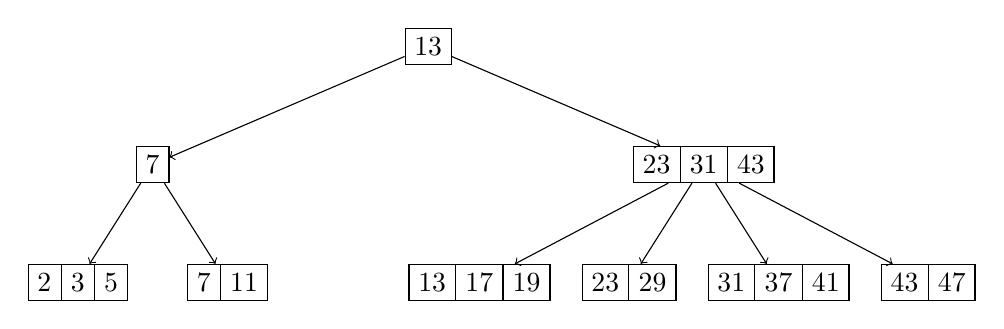
\begin{tikzpicture}
\tikzstyle{bplus}=[
	rectangle split,
	rectangle split horizontal,
	rectangle split ignore empty parts,
	draw ]
\tikzstyle{every node}=[bplus]
\tikzstyle{level 1}=[sibling distance=70mm]
\tikzstyle{level 2}=[sibling distance=19mm]
\node {13} [->]
	child {node {7}
    child {node {2 \nodepart{two} 3 \nodepart{three} 5}}
    child {node {7 \nodepart{two} 11}}
  }
  	child {node {23 \nodepart{two} 31 \nodepart{three} 43}
  	child {node {13 \nodepart{two} 17 \nodepart{three} 19}}
  	child {node {23 \nodepart{two} 29}}
  	child {node {31 \nodepart{two} 37 \nodepart{three} 41}}
  	child {node {43 \nodepart{two} 47}}
  }
;
\end{tikzpicture}
\end{center}

\begin{quote}
$i.$ Draw the B-tree after deleting 7. \\
$ii.$ After $i$, draw the B-tree after deleting 17. \\
$iii.$ After $ii$, draw the B-tree after deleting 43. \\
$iv.$ After $iii$, draw the B-tree after inserting 51. \\
$v.$ After $iv$, draw the B-tree after inserting 32.
\end{quote}

\vskip.35in
\noindent{\textbf{Section 5: Essay [10 points]}}

\vskip.10in
\noindent Use your own words to explain the following:

\begin{quote}
$i.$ What are benefits to having shared locks? \\
$ii.$ What does a scheduler do and what is scheduling latency? \\
$iii.$ What is throughput and what are ways to increase it? \\
$iv.$ What are different ways for a disk to fail? \\
$v.$ What are the usual tradeoffs to consider when normalizing relations?
\end{quote}

\begin{center}
\vspace{3cm}
\textit{\lastwords}
\end{center}

\label{finalpage}


\end{document}
